\section{Background}

In this chapter, the aim is to provide sufficient background information, in order to understand how the cuff-less estimation of blood pressure (BP) values 
can be achieved. An overview on all necessary fields will first be given. These fields are as follows:
\begin{itemize}
  \item Medical Background
  \item Cuffless methods for deriving blood pressure
  \item Neural Networks
  \item Overview on cuffless blood pressure device options
\end{itemize}\noindent Finally, a literature review will be conducted to 
assess what is the most feasible implementation for blood pressure cuffless estimation for this FYP.

\subsection{Medical background}
In this chapter, all of the medical knowledge required to 
understand the basis of this project will be discussed.
\subsubsection{Hypertension}
The heart can suffer from a variety of diseases and pathologies. Low blood 
pressure, or hypotension, has the potential to cause  a lack of oxygen 
flowing to the  brain  and  other  organs, causing shock \cite{Tanveer2018}. 
Whilst hypotension is a serious issue, hypertension has been identified by 
the World Health Organization (WHO) as the most significant risk factor for 
cardiovascular diseases \cite{Wang2018}. According to the 2017 American Heart 
Association guidelines for hypertension, the risk of developing stage two 
hypertension, $\ge 140$ mmHg systolic or $\ge 90$mmHg diastolic is almost 
90\% \cite{Bard2019} (see Table \ref{bp_vals_table}). Over 20\% of adults have 
hypertension  and  its  complications  cause  a  major  number  of  
diseases, including heart attacks, strokes and heart failure. If 
hypertension is not diagnosed and properly treated it can even cause 
death \cite{Janjua2017}.\\ \newline \noindent  Hypertension or high blood pressure (BP) is where blood continues to exert more and more pressure on the arterial walls. One particular disease linked to hypertension is hypertrophic cardiomyopathy, as indicated in Figure \ref{hypertension}, \begin{figure}[H]
    \centering
    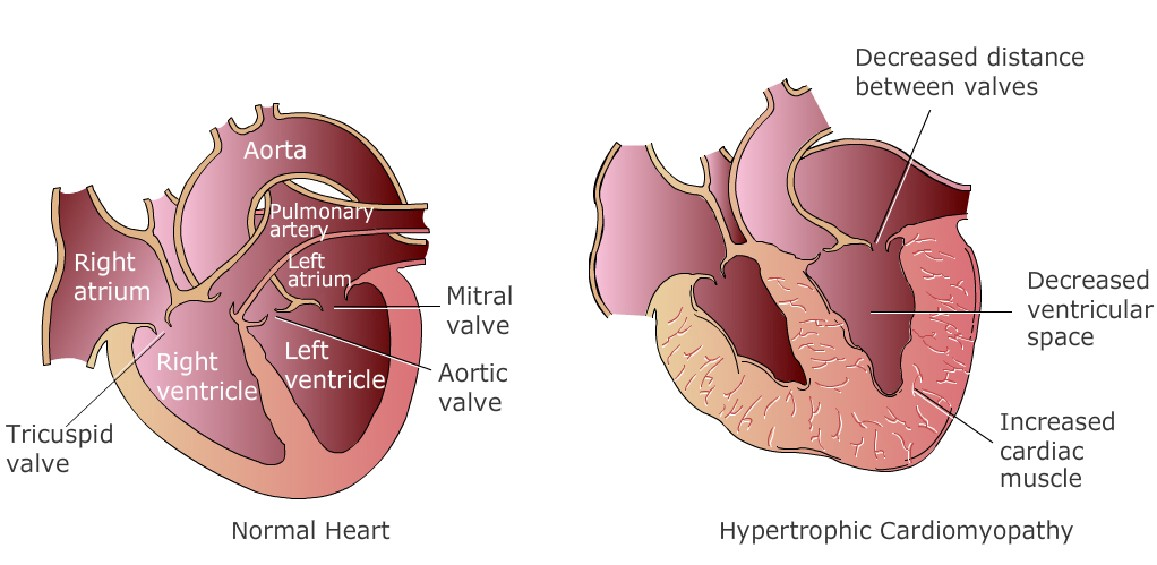
\includegraphics[width=12cm,height=12cm,keepaspectratio]{Background/hypertension.jpeg}
    \caption{The effects of hypertension on the heart \cite{hypertrophic}}
    \label{hypertension}
\end{figure} \noindent Hence it is clear that hypertension is one of the largest motivating factors for this project.

\begin{table}[H]
    \centering
    \caption{Categories of blood pressure in adults \cite{Wang2018} \cite{Simjanoska20181}}
\begin{tabular}{|c|cc|}
\hline
\multirow{2}{*}{\textbf{Blood pressure classification}} & \multicolumn{2}{c|}{\textbf{Blood Pressure (mmHg)}} \\
 & \textbf{Systolic} & \textbf{Diastolic} \\ \hline
Hypotension & $\le$ 90 & Or $\le$ 60 \\
Normal & 90-119 & And 60-79 \\
Prehypertension & 120-139 & Or 80-89 \\
Stage 1 hypertension & 140-159 & Or 90-99 \\
Stage 2 hypertension & $\ge$ 160 & Or $\ge$ 100 \\ 
Isolated Systolic hypertension & $\ge$ 140 & And $<$ 90\\
Hypertensive crisis & $\ge$ 180 & Or $\ge$ 110 \\ \hline
\end{tabular}
\label{bp_vals_table}
\end{table}

\subsubsection{Ambulatory Blood Pressure (ABP)}
ABP monitoring (ABPM) is when BP is measured as the patient moves around, and it allows 
patients to still live their normal daily lives \cite{Huang2021}. It has been 
classed as the gold standard for detecting and diagnosing hypertension and 
also assessing BP values over a 24 hour period \cite{Kario2021}. ABPM provides 
data on several important and unique parameters \cite{Kario2021}. This data can
 explain how changes in your BP may correlate with your daily activities and sleep 
 patterns \cite{Huang2021}. Conventionally,  ABP is monitored by using a cuff 
 attached to a portable device which is worn on the patient's 
 waist \cite{Kario2021}.

\subsubsection{Blood Pressure measurements} 
Blood pressure (BP) is the force of the blood pushing against the 
arterial walls as the heart pumps blood. It is measured in millimeters of 
mercury (mmHg) \cite{Simjanoska20182}. BP  is  measured  in  terms  of  
systolic  blood  pressure  (SBP)  and  diastolic  blood  pressure  
(DBP). These values are the maximum and minimum pressure values of an 
Arterial Blood Pressure waveform during a cardiac cycle 
respectively \cite{Simjanoska20181} \cite{Pradenas2020}. An example of this structure is provided in Figure \ref{abp}.
\begin{figure}[H]
   \centering
   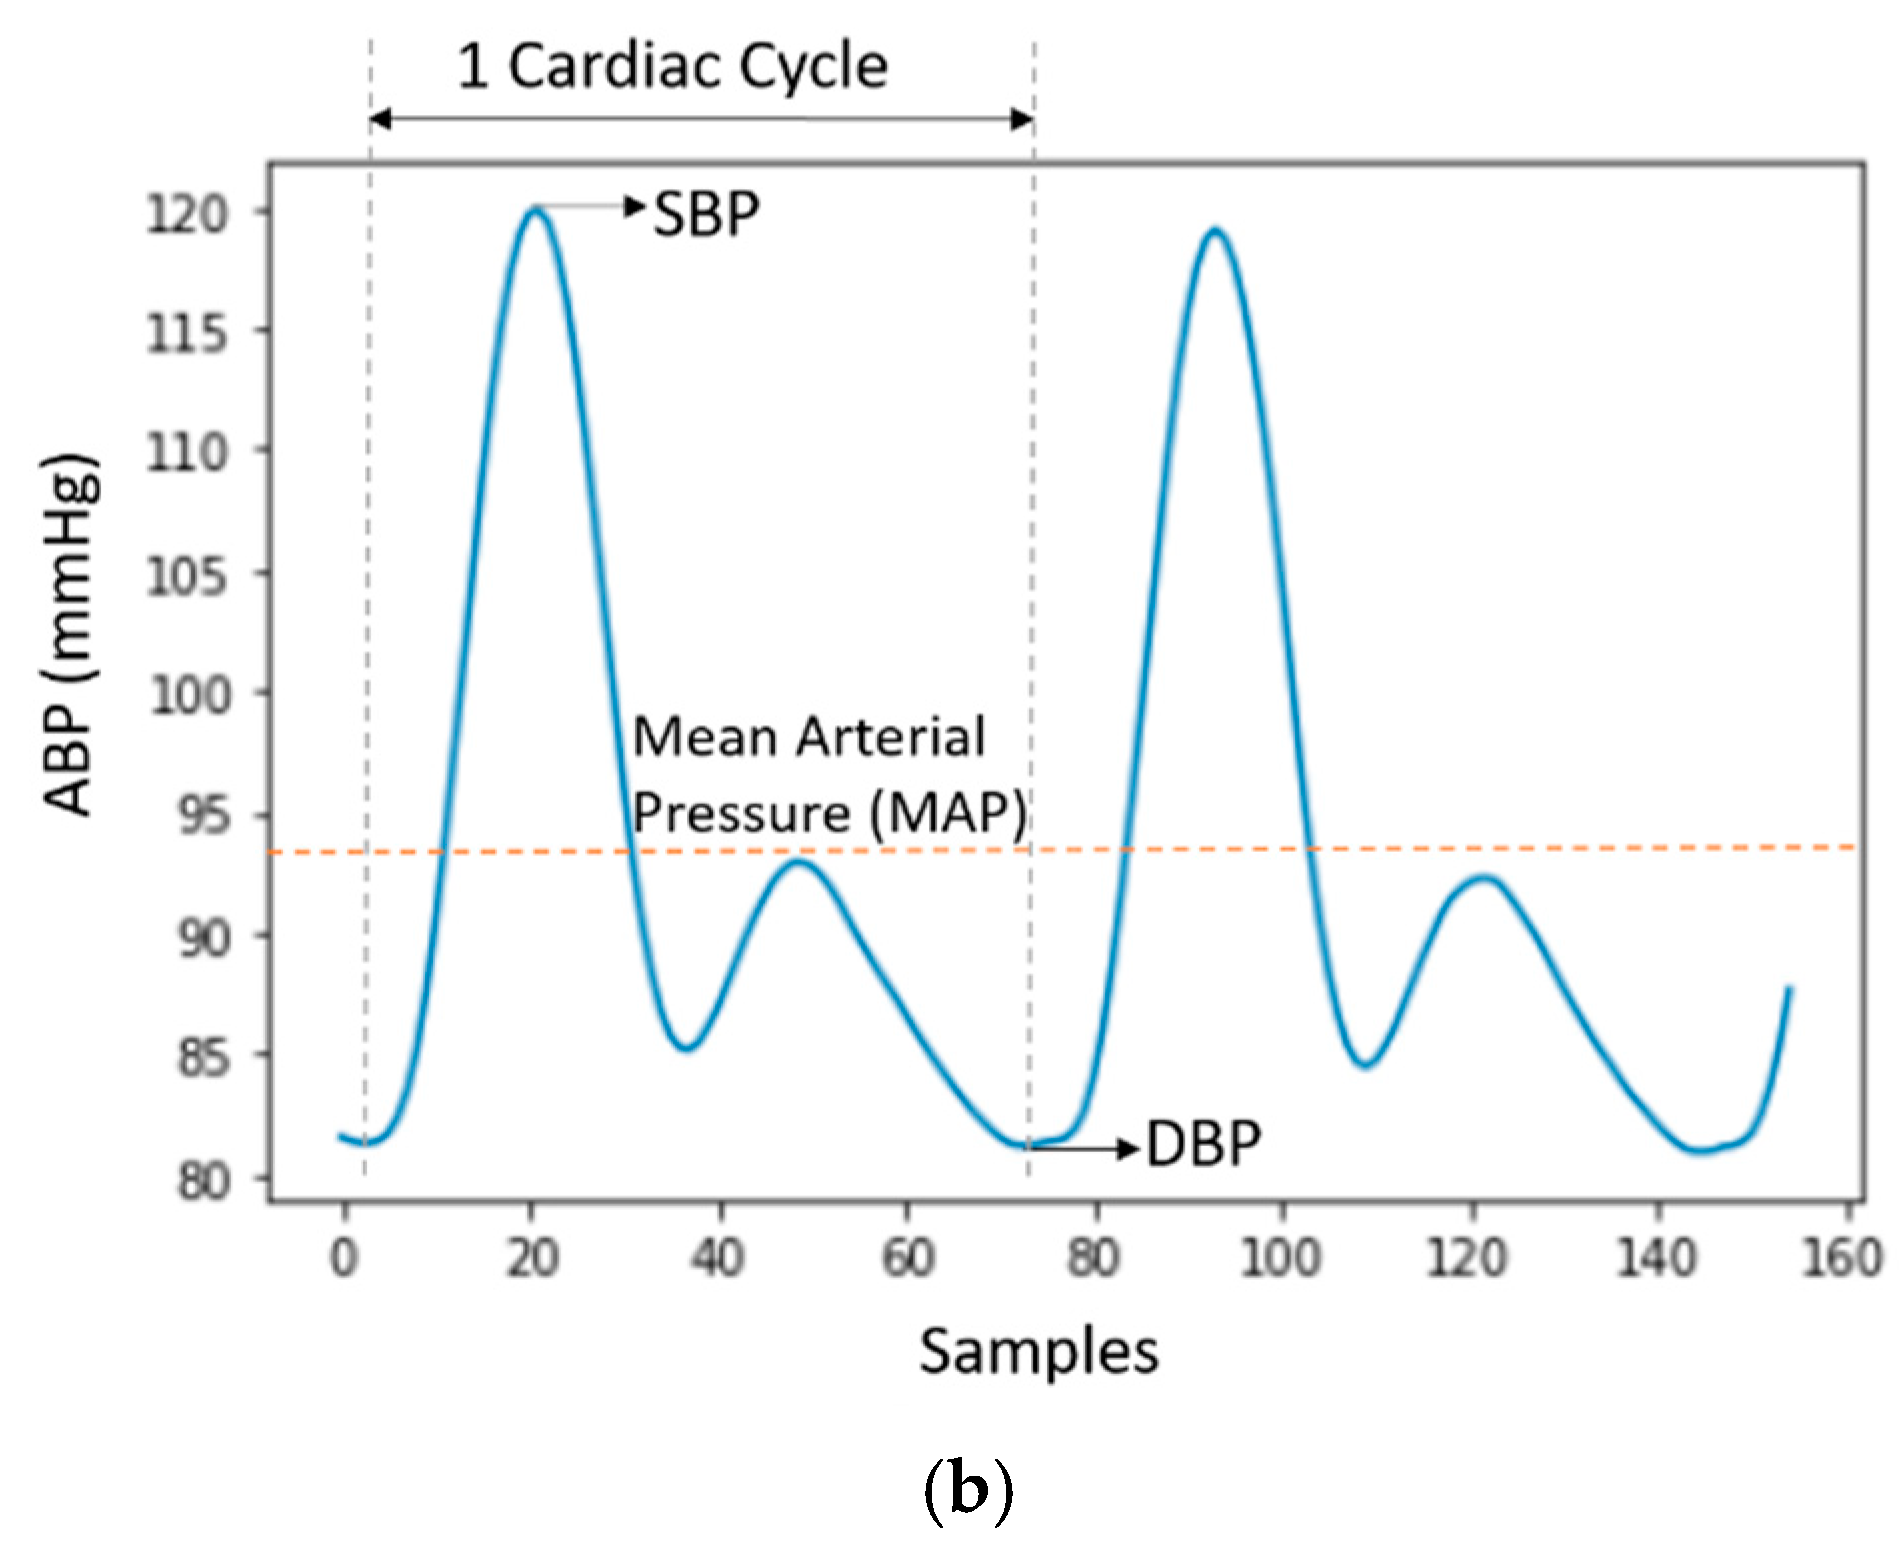
\includegraphics[width=12cm,height=12cm,keepaspectratio]{Background/abp.png}
   \caption{Structure of an Arterial Blood Pressure signal \cite{Athaya2021}}
   \label{abp}
\end{figure}\noindent As shown in Figure \ref{abp}, the Systolic and Diastolic Blood Pressure 
values of the waveform are defined by the maximum and minimum ABP values within the provided 
sampling window. \\ \newline \noindent BP  has 
oscillations or pulses that mirror the oscillatory nature of the heart. The blood is 
propelled during systole, also known as heart contraction, and the blood is  
rested during  diastole, known as heart  relaxation, as illustrated in Figure \ref{diastoleSystole}. \begin{figure}[H]
    \centering
    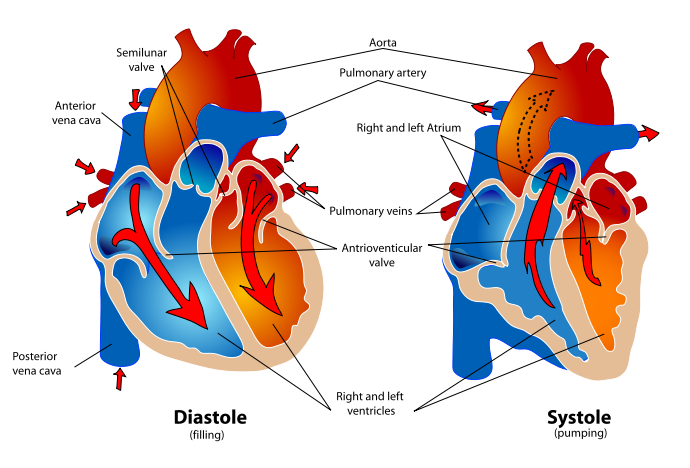
\includegraphics[width=12cm,height=12cm,keepaspectratio]{Background/sbp_dbp.png}
    \caption{Visualisation for SBP and DBP \cite{SBP}}
    \label{diastoleSystole}
\end{figure}\noindent Blood pressure values can also be assessed mathematically using the following formulae \cite{Shaffer2017},
\begin{align}
    \text{Normal-to-normal (NN) interval } &= \frac{\text{Largest difference between systolic peaks}}{f_s}\\
    \text{Heart rate (HR) } &= \frac{60}{\text{Mean (NN interval)}} 
\end{align}\noindent where $f_s$ is the sampling frequency of the signal. \\ \newline \noindent There 
are two  conventional  methods  for  measuring  blood  pressure (BP). These 
are invasive   and   non-invasive methods. \\ \newline \noindent  The most popular form of invasive  BP 
measurement is  catheterization \cite{Zaki2018}. Invasive BP measurements 
are continuous and the most accurate from heartbeat to heartbeat. As a result 
these measurements are recognised as the gold standard 
internationally \cite{Sharma2017} \cite{ElHajj2020}. However, this method is 
usually restricted to hospitals, as medical supervision is required \cite{Pradenas2020}. 
In addition, this method poses several health risks, including bleeding and 
infection. As a result, invasive measurements are only utilised for critically 
ill patients in intensive care units and for use during 
surgery \cite{Zaki2018}\cite{ElHajj2020}. The main form of non-invasive BP measurements are through 
upper arm cuffed monitors. These forms of measurements are more beneficial than the invasive gold standard 
method, because they do not cause any major health risks \cite{ElHajj2020}. However, 
if the cuff is worn on the arm for extended periods of time, this will cause a lot of 
discomfort to the patients \cite{Tanveer2018}. In addition, it has been found that over three in ten home BP monitoring 
cuffs have produced inaccurate results \cite{Leung2016}. \\ \newline \noindent  As a 
result, the existing invasive and non-invasive BP measurement techniques are not 
feasible for an implementation involving continuous ambulatory BP 
monitoring \cite{ElHajj2020}. Hence, after having assessed the viability of all 
aforementioned methods, it is clear that it is difficult for these methods to be 
integrated with wearable technologies, which continue to gain popularity in 
commercial sectors and clinical practice \cite{Sharma2017}. This provides the motivation in using 
other heart signals which do not require invasive or cuff-based methods to be measured accurately.

 \subsubsection{Electrocardiogram (ECG) signals} 
 ECG signals provide an overview of the electrical impulses occurring in the 
 heart \cite{Simjanoska20181}. Electrical changes in the heart conduct
  through the body and are received at skin level. The record of these
   electrical fluctuations during the cardiac cycle is called the 
   Electrocardiogram (ECG) \cite{Kumar2015}. The signals are recorded 
   by measuring the electric potential difference by placing electrodes 
   across the heart of an individual \cite{Tanveer2018} \cite{Simjanoska20181}. 
   These electrodes are connected to the ECG machine with recordings from 12 
   different places on the body, which is known as the 12-lead ECG. The standard 
   ECG leads are I, II, III, aVF, aVR, aVL, V1, V2, V3, V4, V5, V6. Leads I, II, 
   III, aVR, aVL, aVF are classed as the limb leads and the others are 
   precordial leads \cite{Tanveer2018}. \\ \newline \noindent The QRS complex 
   of an ECG signal is detailed in Figure \ref{qrs}. This complex is first 
   created through the generation of the electrical impulses from the heart. 
   These signals then move along the electrical highway and as a result cause 
   the ventricles to contract and pump oxygenated blood into the arteries. 
   Physically, this whole describes the QRS 
   complex \cite{Kumar2015}. \begin{figure}[H]
    \centering
    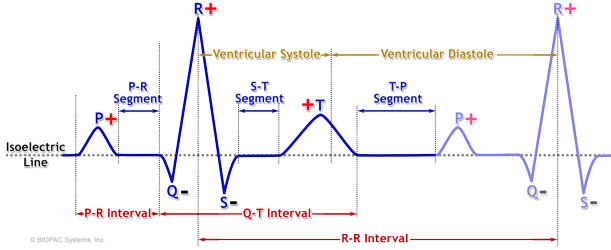
\includegraphics[width=12cm,height=12cm,keepaspectratio]{Background/qrs.png}
    \caption{Structure of an ECG signal \cite{ecgWiki} \cite{qrsWiki}}
    \label{qrs}
\end{figure}



\subsubsection{Photoplethysmography (PPG) signals} 
Photoplethysmography (PPG) measures the blood volume changes per pulse. It is an optical and non-invasive 
technique that can determine a wide range of medical values, including an estimate for BP \cite{ElHajj2020}. 
Physically, the PPG signal is acquired by measuring the optical signal transmitted through or reflected  
from  the  subject's tissue \cite{Tanveer2018}. The PPG sensor consists of two components. The first component 
is an Light Emitting Diode (LED) to light up the surface of the skin. The second component is a photodetector, 
which is utilised for measuring the changes in light absorption over a period of time \cite{ElHajj2020} \cite{Kumar2015}.
\begin{figure}[H]
    \centering
    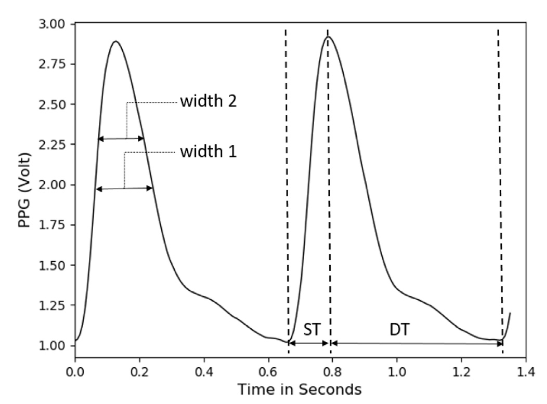
\includegraphics[width=12cm,height=12cm,keepaspectratio]{Background/ppg.png}
    \caption{Structure of a PPG Signal \cite{ElHajj2020}}
    \label{ppg}
\end{figure} \noindent In Figure \ref{ppg}, the four features 
are the Systolic upstroke Time (ST), Diastolic Time (DT), 
width at $\frac{1}{2}$ amplitude (width 1) and width at $\frac{2}{3}$ 
amplitude (width 2) \cite{ElHajj2020}. PPG waveforms have a wide range of 
temporal features \cite{ElHajj2020}. These features have been utilised 
in several experimentations, creating  models  to  estimate blood 
pressure \cite{Pradenas2020}.


\subsection{Cuff-less methods for deriving blood pressure (BP)} 
Cuff-less  methods have great potential in being used to estimate BP. 
This is because they provide continuous measurements, they cause minimal 
harm to the patients and they produce BP values over a long period of 
time  \cite{Liu2020}. There are three fundamental cuff-less methods 
which will now be discussed which can be used for deriving BP. These 
three methods rely on Pulse Transit Time (PTT), Pulse Arrival 
Time (PAT) and Pulse Wave Velocity (PWV) respectively \cite{Nye2015}. These 
will each now be discussed in more detail.

\subsubsection{Pulse Transit Time (PTT)} 
PTT is the time required for the arterial pressure wave to travel from the 
left ventricle to a distal arterial site. PTT holds an inverse relationship 
to blood pressure and as a result it is dependent on arterial compliance, 
arterial wall thickness, arterial radius, and blood density. PTT is 
conventionally found with the use of two PPG 
sensors \cite{Tanveer2018} \cite{Wang2018} \cite{ElHajj2020}, as indicated 
in Figure \ref{ptt}.
\begin{figure}[H]
    \centering
    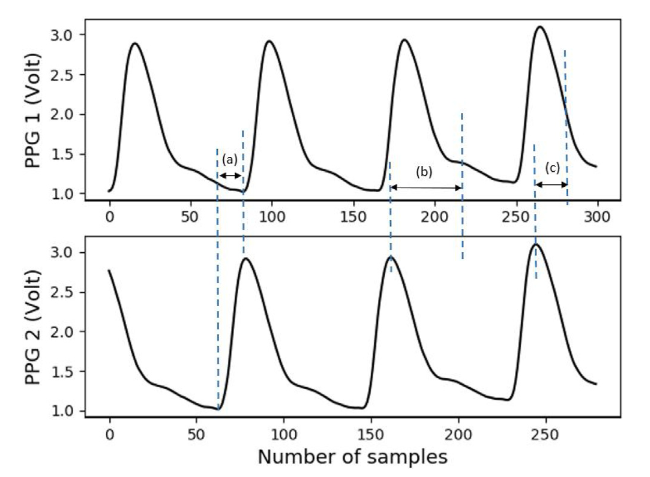
\includegraphics[width=12cm,height=12cm,keepaspectratio]{Background/ptt.png}
    \caption{Pulse Transit Time (PTT) visualisation \cite{ElHajj2020}}
    \label{ptt}
\end{figure} \noindent It is important to note for 
Figure \ref{ptt} that the PTT can be measured at different points along 
the PPG waveforms. (a) represents a foot-to-foot time delay, (b) is a 
peak-to-dicrotic notch time delay and (c) is a peak to mid-point of the 
falling edge time delay \cite{ElHajj2020}. As a proof of concept, increasing 
blood pressure leads to an increase in the tension along the arterial wall tension, which 
therefore reduces the PTT. Hence, the opposite also applies \cite{Kumar2015}.

\subsubsection{Pulse Arrival Time (PAT)} 
The PAT is the difference in time between the R-peak of the ECG signal and 
the systolic peak of the PPG signal when measured during the same 
cardiac cycle, as indicated in 
Figure \ref{pat} \cite{ElHajj2020} \cite{Malikeh2019}. Physically, 
PAT is the interval in time between the activation of electrical 
impulses at the heart and the arrival of the pulse wave at a location 
on the body, such as the finger \cite{Jeong2021}. PAT is measured using 
two sensors, an ECG and a PPG sensor \cite{ElHajj2020}. 
\begin{figure}[H]
    \centering
    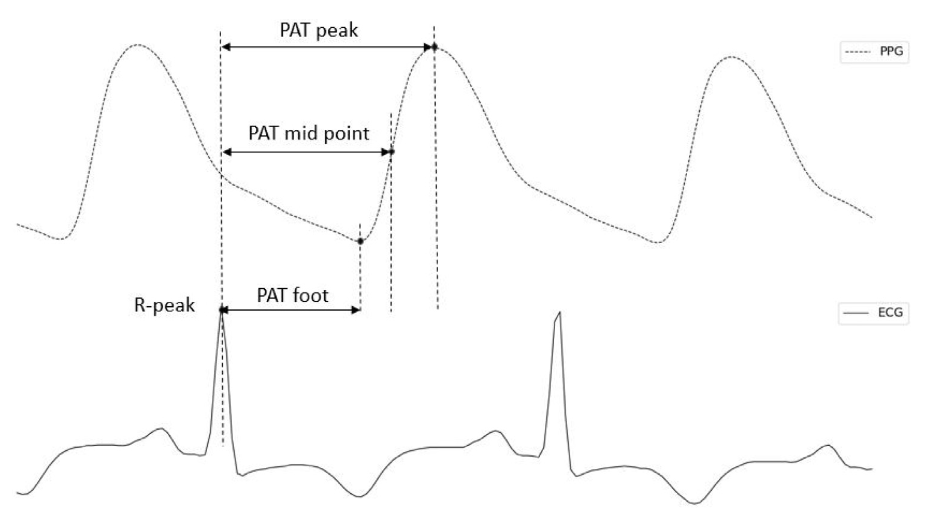
\includegraphics[width=12cm,height=12cm,keepaspectratio]{Background/pat.png}
    \caption{Pulse Arrival Time (PAT) visualisation \cite{ElHajj2020}}
    \label{pat}
\end{figure} \noindent The Pre-ejection Period (PEP) delay can 
also be briefly discussed. PEP is the time needed to convert the electrical 
signal into a mechanical pumping force and isovolumetric contraction to open 
the aortic valves, 
\begin{align}
    PAT = PTT + PEP
\end{align}

\subsubsection{Pulse Wave Velocity (PWV)}
The PWV calculates the velocity of the pulse wave using two PPG sensors 
located on the same arterial branch at a known distance 
apart \cite{Pradenas2020} \cite{ElHajj2020}. The relation between PTT 
and PWV can be expressed as 
\begin{equation}\label{eq_pwv1}
    PWV = \frac{d}{PTT}
\end{equation} where $d$ is the arterial distance travelled by the pressure 
wave. PWV is related to the Young's modulus of the vessel wall by the 
Moens-Kortweg equation, 
\begin{equation}\label{eq_pwv2}
    PWV = \sqrt{\frac{Eh}{\rho d}}
\end{equation} where \\ \newline \noindent 
\begin{flalign}
        PWV &= \text{ Velocity of the pulse wave (m/s)} &\\
        E &= \text{ Young's modulus of vessel wall (Pa)} &\\
        h &= \text{ vessel thickness (m)} &\\
        \rho &= \text{ blood density (kg/$m^3$)} &\\
        d &= \text{ arterial diameter (m)} &
    \end{flalign}\\ \newline \noindent The Young's modulus of the 
vessel wall is then related to the arterial pressure by the 
Bramwell-Hills equation, 
\begin{align}
    E = E_0 e^{\lambda P}
\end{align}where $E_0$ and $\lambda$ depend  on  the  thoracic  and 
abdominal aortas and P is the vessel blood pressure 
(mmHg) \cite{Janjua2017} 
\cite{Tanveer2018} \cite{Yang2020}. \\ \newline \noindent By equating and solving 
Equations \ref{eq_pwv1} and \ref{eq_pwv2}, the final equation for estimated 
blood pressure is expressed as, \begin{align}
    P = \frac{1}{\lambda} \ln{(2 r \rho \frac{\Delta X^2}{E_0 h})} - \frac{2}{\lambda} \ln{(PTT)}
\end{align} \\ \newline \noindent where 
\begin{flalign}
    r &= \frac{d}{2} = \text{ arterial radius} &\\
    \Delta X &= \text{ distance from heart to vessel} &
\end{flalign}

\subsubsection{Limitations}
Blood pressure (BP) can be derived through mathematical models as 
soon as estimates have been calculated for PTT, PAT and PWV. Although 
these models are common approaches for BP monitoring in an environment 
that is non-invasive and cuff-less, there are many challenges to these 
implementations. As a result, none of these techniques by themselves 
have been established as a reliable indicator for the estimation 
of BP. \\ \newline \noindent Firstly, all three of the aforementioned 
methods require two separate measurements from two synchronised sensor 
devices. This can be a very inconvenient process for patients who are
uncomfortable with this method \cite{Jeong2021}. In 
addition, there is a very likely possibility that these sensor devices 
will have different real-time sampling rates. In order to be able to 
continuously measure BP, constant calibration of the methods is 
required \cite{ElHajj2020}. This is due to individual patients having different 
physiological parameters \cite{Jeong2021}. Finally, 
even with per-person calibration, these models can only provide BP 
estimation for a short period of time. As a result, this makes the 
models unreliable for the estimation of BP with every 
heartbeat \cite{ElHajj2020}. \\ \newline \noindent To conclude this 
chapter, there is a lot of potential in the use of the three above 
parameters in the estimation of Ambulatory BP. However, there are still 
overarching limitations which currently hinder the progress of estimation using these 
parameters. As a result, the use of these parameters is not recommended for investigations which 
involve signal data over a long period of time, due to data processing limitations. This provides the motivation to use data-driven techniques, as discussed in the next 
section.




 \subsection{Neural Networks}

 In this section the aim is to describe neural networks in a number of stages. Firstly, an overview of why they form part of a field 
 of data-driven techniques is given and how the complexity of the calculations are affected. Finally, all other parameters important to defining neural network architectures will be defined.

 \subsubsection{Artificial neural networks}
 Artificial Neural Networks (ANNs) are a family of data-driven techniques. These techniques are 
 successfully able to automatically extract features from the input data, instead of creating and solving a system of equations, as seen in the previous section. Due to advancements in technology related to machine learning, there has 
 been a lot of research into neural networks algorithms that can offer 
 continuous BP measurements that are non-invasive and also 
 cuffless \cite{Pradenas2020}. However, in this case BP 
 estimation is motivated by how much data is available to the 
 algorithm \cite{ElHajj2020}. \\ \newline \noindent Artificial neural 
 networks (ANNs) are a machine learning method that can be used to estimate 
 blood pressure \cite{Pradenas2020}. ANNs are based on the neural networks 
 found in the human body and aim to replicate their behaviour \cite{Yang2020}. The 
 structure of the ANN consists of multiple individual units called neurons. A single neuron is shown in Figure 
 \ref{neuron}.  \begin{figure}[H]
    \centering
    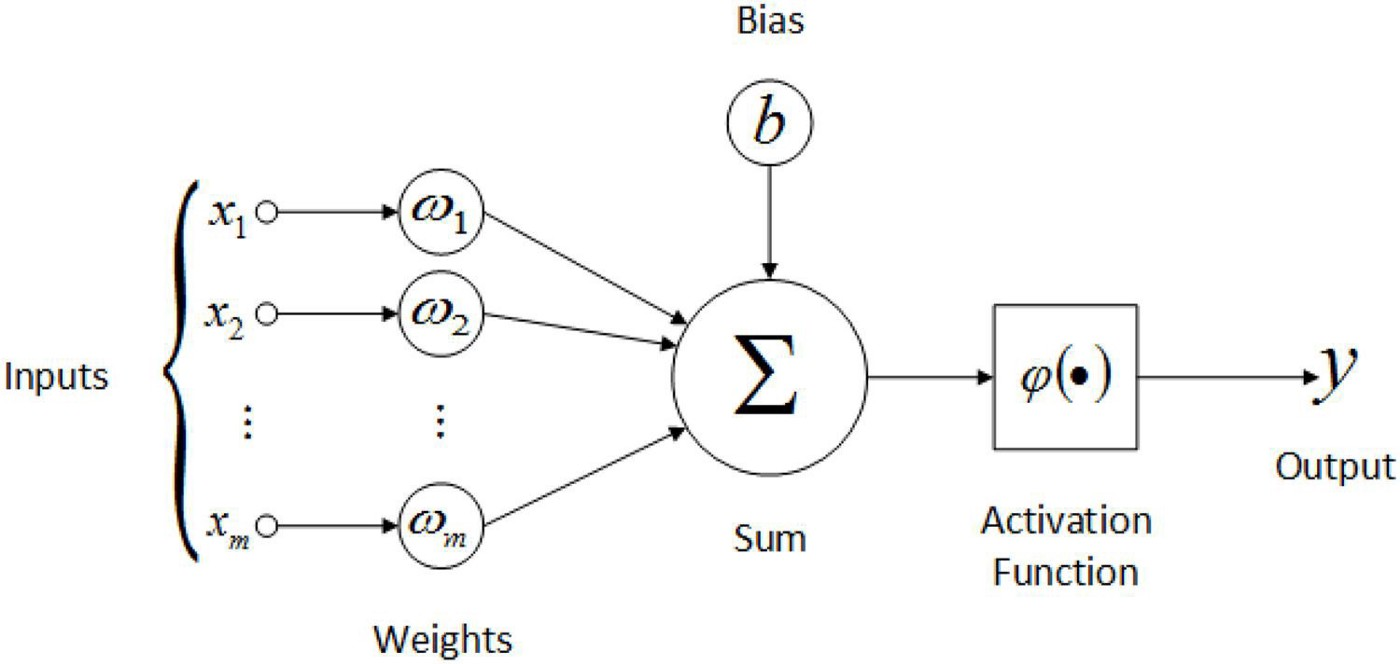
\includegraphics[width=10cm,height=10cm,keepaspectratio]{Background/neuron.jpeg}
    \caption{Structure of a neuron \cite{Almusawi2020}}
    \label{neuron}
\end{figure}\noindent Each 
 neuron has five main building blocks. These are inputs ($\bm{x}$), weights ($\bm{\omega}$), transfer 
 function ($\Sigma$), activation function ($\phi(\cdot)$) and bias ($b$) \cite{deeplearning}. In order to mathematically 
 express the neuron unit, it is important to first understand its goal. The neuron
 applies a dot product with the weights $\bm{\omega}$ and 
adds a scalar bias $b$. After this, a non-linear 
activation function $\phi(\cdot)$ is applied, which enables non-linear relationships, such as those 
seen in cuffless estimation of blood pressure, to be modelled. This is expressed mathematically as follows,
\begin{equation}\label{eq_neuron}
    y = \phi(\sum_{i} \omega_i x_i + b ) = \phi (\bm{\omega}^T \mathbf{x} + b)
\end{equation}\noindent where $\bm{\omega} \in \mathbb{R}^m$ 
and $y$, $b$ are scalars. When each of these neurons are connected together with several other 
neurons across several layers, this forms an ANN, as shown in Figure \ref{ann}, where each of the 
neurons are represented by a grey unit. ANNs enable the modelling of more 
complex relationships than just a single neuron. In the case of estimating blood pressure values, this machine learning problem would be treated 
as a regression problem, which is where the aim is to predict a real and continuous value. Ideally, the network will have two regression values 
at the output, one for the Systolic Blood Pressure (SBP) and one for the Diastolic Blood Pressure (DBP). The network of a single fully-connected layer is mathematically expressed using Equation \ref{eq_layer}, 
\begin{equation}\label{eq_layer}
    \mathbf{y} = \phi (\bm{\Omega} \mathbf{x} + \mathbf{b})
\end{equation}\noindent where $\bm{\Omega} \in \mathbb{R}^{N \times M}$ is the weights matrix, 
$\mathbf{b} \in \mathbb{R}^N$ is the bias vector, $\mathbf{y} \in \mathbb{R}^N$ is the output 
vector and $\phi(\cdot)$ performs element-wise non-linear transformations.

 \begin{figure}[H]
    \centering
    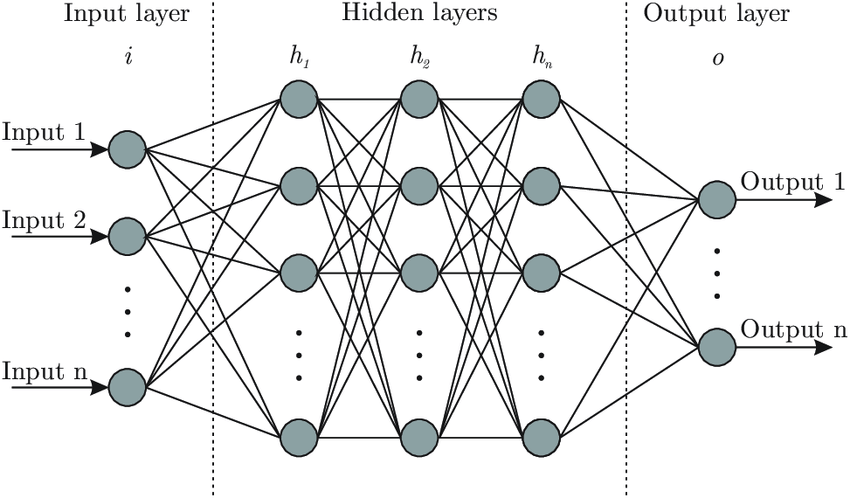
\includegraphics[width=10cm,height=10cm,keepaspectratio]{Background/ann.png}
    \caption{Structure of a multi-layer ANN \cite{deeplearning}}
    \label{ann}
\end{figure}\noindent Convolutional Neural Networks (CNNs) are a specific class of 
ANNs. Two-dimensional CNNs were originally developed for two-dimensional image classification problems. However, for this FYP the CNNs accept one-dimensional data inputs. 
CNNs and all other neural network architectures can either be given specific of the data as input or can be given the whole dataset to learn from. In the second case, the neural network 
itself extracts the strongest features from the data in order to make accurate estimations. Three high performing one-dimensional CNN models are the AlexNet \cite{alexNet}, ResNet \cite{resnetArch} and 
ResNet-LOSO (Leave One Subject Out) \cite{slapnicar2019} architectures.

 \subsubsection{Recurrent Neural Networks (RNNs)}
 Although CNNs have the potential to extract features from time-series data, they face issues as the input sizes increase. Larger sizes result in a much longer time in 
 training on the data, leading to large increases in computational complexity. A Recurrent Neural Network (RNN) is a specific type of architecture that is 
 widely used to deal with time-varying data \cite{rnns}. RNNs contain additional memory states that retain and process information from previous
 time steps.\\ \newline \noindent RNNs are called recurrent since 
 they apply the same operation to each of the input sequences, with the output 
 of an individual element being dependent on the previous one. Theoretically, 
 RNNs establish a connection between the actual input and all the previous 
 ones \cite{rnns}. Although this is assumed, in the practice, RNNs have 
 proven to only remember a limited number of inputs. In other words, RNNs 
 have a memory that allows them to remember previous elements and use their 
 information to deal with the current 
 input \cite{deeplearning}. \noindent Figure \ref{rnn2} shows the simplest version 
of an RNN, which can be easily derived from a simple feedforward architecture by 
adding a single loop:
\begin{figure}[H]
    \centering
    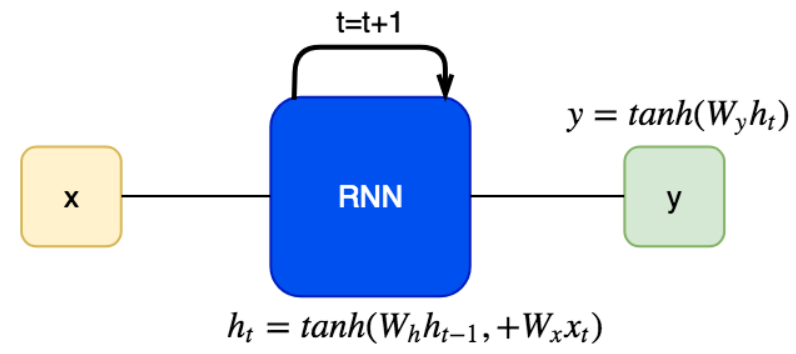
\includegraphics[width=15cm,height=15cm,keepaspectratio]{Background/rnn2.png}
    \caption{Simplification of a RNN  \cite{deeplearning}}
    \label{rnn2}
\end{figure} \noindent During training, the hidden state $h$ is 
iteratively updated based on the input value $x$ and the learned weights $W_h$  
and $W_x$. The final output $y$  is estimated from the current state $h_t$  
and the matrix $W_y$. Although RNN can assure short-term dependencies within 
the network, simple RNNs become unable to learn to connect information as the 
gap between past and present information grows \cite{lstm}. This is known as the vanishing gradient problem. To overcome this 
limitation, in practical applications the Long Short Term Memory (LSTM) unit is adopted. This is a special 
RNNs architecture composed of multiple interacting layers.
\begin{figure}[H]
    \centering
    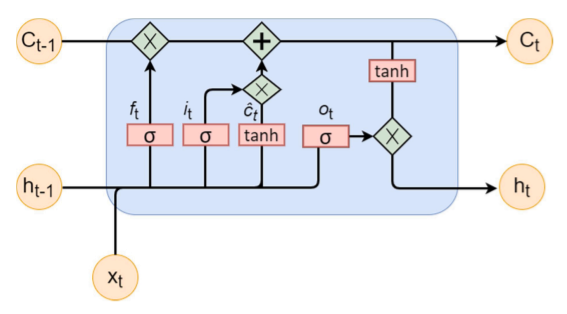
\includegraphics[width=15cm,height=15cm,keepaspectratio]{Background/rnn3.png}
    \caption{Structure of an LSTM cell \cite{ElHajj2021}}
    \label{rnn3}
\end{figure}\noindent As previously noted, LSTMs are more efficient than the standard RNNs 
in processing sequential data, as they are able to learn long-term dependencies in the data, which 
effectively removes the vanishing gradient problem seen in RNNs. There are two other main variants of LSTMs. Firstly the Gated Recurrent Unit (GRU), which uses fewer parameters and does not have an output gate in comparison 
with the LSTM, and the Bi-directional LSTM (Bi-LSTM), which is able to process the sequential input data in both the forwards and backwards direction.

\subsubsection{Transformers}

Transformers are another class of ANN that provide state-of-the-art solutions 
for many of the problems previously assigned to RNNs \cite{transformers}. Transformers 
were originally created for solving problems in Natural Language Processing (NLP) but can 
also be extended to time-series sequential data. Unlike RNNs and their variants, transformers do not 
use any recurrent connections and hence have no memory of previous data during training. However, transformers solve this problem 
by processing whole segments of sequential data at a time. As a result of this, the depth of the neural network is reduced, leading to 
a decrease in computational complexity. For the purposes of this FYP, the focus will be on the transformer encoder 
architecture. The main building block of a transformer encoder is the Encoder block, which is represented as a block diagram in Figure \ref{transformer}.
\begin{figure}[H]
    \centering
    
\includegraphics[width=15cm,height=15cm,keepaspectratio]{Background/transformer.png}
    \caption{Block diagram to illustrate the Encoder block \cite{transformers}}
    \label{transformer}
\end{figure}\noindent The following stages are described as follows:

\begin{itemize}
    \item \textbf{Layer Normalisation}: applies a normlisation operation across the whole layer of data inputs
    \item \textbf{Self-Head Attention}: performs 3 main tasks; firstly it performs a dot product similarity to find alignment scores, then performs normalization of the scores to get the weights and finally reweighs the original embeddings using the weights
    \item \textbf{Feed Forward Neural Network}: 1-dimensional CNN that processes the data from the output of the attention block
\end{itemize}\noindent It is important to note that the main limitation of transformers is that 
they require a lot of data to learn effectively \cite{transformers}. Having provided an overview of three families of neural networks, it is now necessary to introduce a few additional concepts for the purposes of this FYP.

\subsubsection{Activation Functions}
Activation functions are able to model non-linear functions by applying a non-linear mathematical operation to the input. For this project, the estimation of BP is treated as a regression problem. 
Hence, the rectified linear unit (ReLU) activation function is ideally used during the training process, and is mathematically described as follows,
\begin{equation}
    f(x) = \max(0,x)
\end{equation}\noindent where $f$ is the output of the ReLU activation function 
and $x$ is the input.

 \subsubsection{Loss Functions}
 During the training process of neural networks, their aim is to minimise their loss functions, so that they can achieve the best possible estimation accuracy. For this project, the loss function of concern is the Mean Squared Error (MSE) loss function, which is defined in 
Equation \ref{eq_mse}.
\begin{equation}\label{eq_mse}
    l_\text{MSE }(\mathbf{y}, \mathbf{\hat{y}}) = \frac{1}{N} \sum_{i=1}^N (\mathbf{y}_i - \mathbf{\hat{y}_i})^2
\end{equation}\noindent where $N$ is the number of training examples, $\mathbf{y}_i$ is the target output vector, and $\mathbf{y}_{\hat{y}_i}$ is the predicted output vector. The MSE loss function was chosen, as it has been proven to be more robust to outliers in the predictions by applying larger penalty weights through the squaring operation. The training 
process is finishing after finding the optimal weights (per layer) of the model as expressed in Equation \ref{eq_weightOpt}, where $\mathbf{\hat{y}}$ is the estimate of
 the true label $\mathbf{y}$ and $l$ is the loss function.
 \begin{equation}\label{eq_weightOpt}
    \mathbf{\Omega}_{opt} = \arg \min_{\mathbf{\Omega}} \{\mathbb{E}(l(\mathbf{y}, \mathbf{\hat{y}}))\}
 \end{equation}\noindent Overfitting occurs when the neural network model performs well on the training input data used 
 but performs poorly on the unseen test data. Overfitting is clearly an indicator 
 of poor performance and can be avoided by introducing a validation dataset, which 
 is just a subset of the training data which is not used by the neural network until the very end 
 of the training process. After training the model on the training data, the learned model can then be 
 evaluated on the validation dataset to give the user an insight as to how well 
 the model performs on a set of unseen data.
 
 \subsubsection{Complexity of neural networks}
 There are two main factors associated with the complexity of neural networks:

 \begin{itemize}
    \item \textbf{Input data}: The larger the size of the input data, the greater the number of neurons are required in the neural network architecture. As a result, this leads to a increase in computational time and hence how long it takes to train the neural network model. Specifically for this project, if a large number of features are extracted from the PPG signals, then the computational complexity will significantly increase 
    \item \textbf{Depth of the model}: The depth refers to how many hidden layers are present in the neural network architecture. As this Chapter on neural networks has progressed, several neural network architectures have been discussed, such as CNNs, RNNs, LSTMs and Transformer Encoders. The depths of the networks are greater for the deep neural networks, such as the CNNs and RNNs. Increasing depth leads to a significant increase in the computational complexity of calcuations. As a result, this leads to increases in both the training and inference times. The inference time is the time taken for the model to make a prediction on the test dataset
 \end{itemize}


\subsubsection{Conclusion}
To conclude this chapter, an overview has been given on the underlying theory behind 
the most popular neural network architectures. The main tradeoffs between these architectures 
is the decision between less complexity, with CNN and RNN architectures, and with maximal 
estimation accuracy, with the Transformer encoder architecture. As a result, it is necessary 
to assess all existing methods for cuffless blood pressure estimation, so that it is possible 
to decide which is the best in achieving the objectives of the FYP.

\subsection{Literature Review}
This chapter provides a detailed account of the literature review conducted for this FYP. 
The literature search equation used will first be discussed. This is then followed by an explanation of the PRISMA 
flow diagram and how it was used to benefit this literature review. To help the reader, 
a table of the scientific papers used in this project is provided. Finally, a critical analysis 
will be given on the literature review and what can be concluded as a result. The aim is to be 
able to justify which is the most feasible method for estimating cuffless blood pressure values.

\subsubsection{Survey Equation}
At the beginning of the FYP, the only information provided was the FYP mission statement (see Appendix Item 10.1) and two 
published papers, \emph{A review of machine learning techniques in photoplethysmography for the non-invasive cuff-less measurement of blood pressure} \cite{ElHajj2020} and 
\emph{Continuous Blood Pressure Estimation From Electrocardiogram and Photoplethysmogram During Arrhythmias} \cite{Liu2020}. These resources pserved as an introduction to both the medical background 
and machine learning knowledge for myself. After reviewing this information, the next step was to perform an informal search of literature databases using keywords 
extracted from the FYP brief. These keywords can be divided into two fields: 
\\ \newline \noindent \textbf{Background knowledge}
\begin{itemize}
    \item "Ambulatory"
    \item "Blood Pressure"
    \item "Electrocardiogram"
    \item "Photoplethysmography"
    \item "Wearable technology"
\end{itemize}\noindent \textbf{Implementation strategy}
\begin{itemize}
    \item "Accuracy"
    \item "Algorithm"
    \item "Computational complexity"
\end{itemize}\noindent These keywords were entered into 3 official literature databases, as shown in Table \ref{tabDatabases}.

\begin{table}[H]
    \centering
    \caption{Official online databases used to conduct the literature review \cite{databasesImperial}}
    \label{tabDatabases}
    \resizebox{\columnwidth}{!}{%
    \begin{tabular}{|c|c|}
    \hline
    \textbf{Literature database}          & \textbf{Description}                                           \\ \hline
    ACM Digital Library                   & The digital library of the Association for Computing Machinery \\
    Engineering Village & Database platform for Physics, Electrical Engineering, Electronics and Computing               \\
    IEEE Xplore         & Digital library containing full text of IEEE journals, conference/meeting papers and standards \\
    National Library of Medicine (Pubmed) & Biomedical and life sciences literature                        \\ \hline
    \end{tabular}%
    }
\end{table}\noindent The ACM Digital Library was chosen to help deepen my understanding of the existing algorithms and programming methods available for estimating 
cuffless blood pressure. Engineering Village provides a wide variety of both signal processing and machine learning based methods for cuffless estimation, whereas the IEEE Xplore 
library gives a detailed insight into machine learning based methods for cuffless estimation. Finally the Pubmed database was chosen to help deepen my understanding of the medical knowledge 
required to perform the literature review.\\ \newline \noindent This informal search enabled a clearer understanding of how the relevant published literature phrased their titles. Based on the findings of the informal search, the following 
literature survey search equation was used to identify the literature that best fits the needs of the FYP requirements. The equation chosen was: 

\begin{itemize}
        \item (Extraction OR Estimation OR Review) AND (Blood OR Arterial OR Ambulatory OR Cuffless) AND (Pressure) AND (ECG OR PPG) AND (Machine Learning OR Signal Processing).
\end{itemize}\noindent Hence, this equation was entered into the four databases displayed in Table \ref{tabDatabases}.


\subsubsection{PRISMA checklist}
After applying the chosen equation to the four databases in Table \ref{tabDatabases}, the next step was to systematically eliminate all papers that 
were not relevant to the aims of the FYP. The Preferred Reporting Items for Systematic Reviews and Meta-Analyses (PRISMA) checklist was used to identify the 
motivations, methods and findings of all published articles relevant to this FYP \cite{prisma}. The process is illustrated in Figure \ref{prisma}.
\begin{figure}[H]
  \centering
  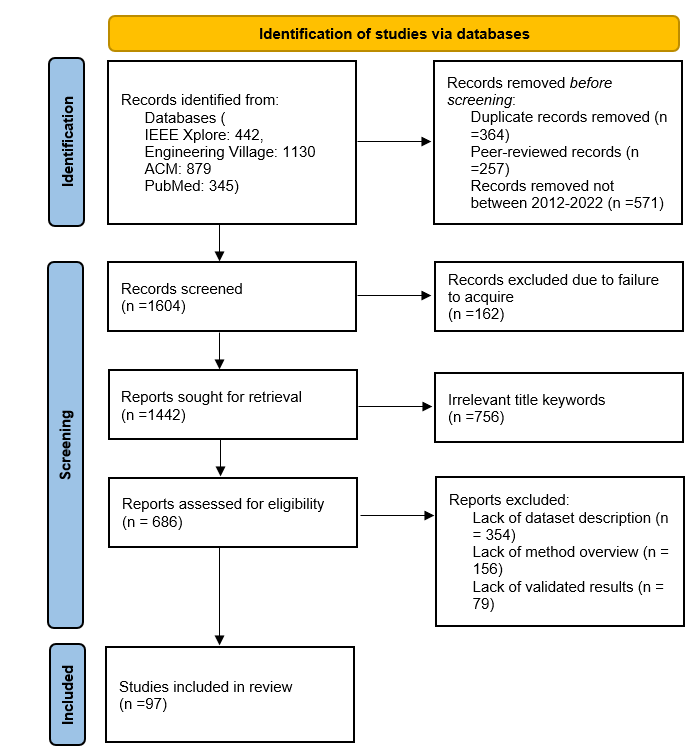
\includegraphics[width=15cm,height=15cm,keepaspectratio]{Background/prisma.png}
  \caption{PRISMA checklist flow diagram (correct to 2020 guidelines) \cite{prisma}}
  \label{prisma}
\end{figure} 

\subsubsection{Literature survey table}
As a reference, the original literature survey matrix can be found on 
the Github repository \cite{LitSurvey}. Firstly, in 
Table \ref{litsurveytab}, a literature survey matrix has 
been detailed out for the best performing methods which do not 
employ machine learning methods. 
\begin{table}[H]
\caption{Overview of performance of the best non-invasive non-ML cuff-less methods for measuring BP}
\resizebox{\columnwidth}{!}{%
\begin{tabular}{|c|c|c|c|c|c|}
\hline
\textbf{Study et al. (Year)} & \textbf{Signal} & \textbf{No. Subjects} & \textbf{Age} & \textbf{Method} & \textbf{MAE SBP} \\ \hline
Ahmad (2012) \cite{Ahmad2012} & ECG, PTT & 10 & 24-63 & Numerical solution & $\pm 5.93$ \\
Chen (2013) \cite{Chen2013} & ECG & 5 & N/A & Analytical solution &  $9 \pm 5.6$\\
Daimiwal (2014) \cite{Daimiwal2014} & PPG & 16 & 18-48 & Frequency analysis &  $0.8 \pm  7$\\
Yamanaka (2016) \cite{Yamanaka2016} & PTT & 127 & N/A & Wavelet transforms &  $\pm 7.63$\\
Ding (2016) \cite{Ding2016} & PTT, PPG & 27 & 21-29 & Analytical solution &  $-0.37 \pm  5.21$\\
Chatterjee (2019) \cite{Chatterjee2019} & PPG & 22 & 22-45 & Cubic regression & N/A\\
Lubin (2020) \cite{Lubin2020} & PPG & 6 & N/A & Analytical solution & N/A\\
Pielmuş (2019) \cite{pielmus2019} & PPG & 10 & $26 \pm 3.3$ & Polynomial regression & N/A\\ \hline
\end{tabular}
}
\label{litsurveytab}
\end{table}\noindent In addition, Table \ref{litsurveytab2} provides an overview of the best performing Machine Learning 
based methods for cuffless estimation of blood pressure values.

\begin{landscape}
    \begin{table}[H]
        \caption{Overview of performance of the best non-invasive ML cuff-less methods for measuring BP}
        \resizebox{\columnwidth}{!}{%
        \begin{tabular}{|c|c|c|c|c|c|}
        \hline
        \textbf{Study et al. (Year)} & \textbf{Signal} & \textbf{No. Subjects} & \textbf{Age} & \textbf{Method} & \textbf{MAE SBP} \\ \hline
        Yang (2020)\cite{Yang2020} & ECG, PPG & 14 males & 17-43 & ANN & $7.99 \pm 10.34$\\
        Gao (2016)\cite{Gao2016} & PPG & 65 & 22-65 & Wavelet, SVM & $5.1 \pm 4.34$\\
        Kachuee (2015)\cite{Kachuee2015} & PPG & MIMIC II & Adults & Linear Reg., ANN, SVM &  $13.84\pm  17.56$\\
        Simjanoska (2018)\cite{Simjanoska20182} & ECG & 51 & 16-83 & Complexity analysis + ML &  $7.72 \pm  10.22$\\ 
        Wang (2018)\cite{Wang2018} & PPG & 72 & N/A & ANN (MLP) & $4.02 \pm 2.79$\\
        Pradenas (2020) \cite{Pradenas2020} & ECG, PPG & MIMIC II & Adults,  neonatal & ANN (150 neurons) & $5.76 \pm 6.39$\\
        Tanveer (2018) \cite{Tanveer2018} & ECG, PPG & 39 & 20-100 & ANN-LSTM & 1.10\\
        Chen (2019) \cite{Chen2019} & PTT, ECG, PPG & MIMIC I & N/A & SVM, Lin Reg. & N/A\\ 
        Ripoll (2019) \cite{Ripoll2019} & PTT & 250 & MIMIC I & ANN-RBM & 3.70\\
        Şentürk (2018) \cite{senturk20181} & ECG, PPG  & N/A (MIMIC II) & N/A & ANN & N/A\\
        Nath (2018) \cite{Nath2018} & PPG & 20 (MIMIC I) & N/A & Random Forest classifier & N/A\\
        Maqsood (2021) \cite{maqsood2021} & PPG & 219 & 21-86 & Bi-LSTM & $3.87 \pm 4.79$\\
        Li (2021) \cite{Li20211} & PPG & 8000 & N/A & PAT features & $4.881 \pm 5.537$\\
        Shimazaki (2018) \cite{Shimazaki2018} & PPG & 1363 & 38-75 & Autoencoder & N/A\\ 
        Şentürk (2018) \cite{senturk20182} & PPG, ECG & N/A & N/A & Bi-LSTM & N/A \\ 
        Xie (2018) \cite{xie2018} & PPG & 11492 & N/A & Random Forest & $4.21 \pm 7.59$\\
        Li (2020) \cite{Li20212} & PPG, ECG & 12000 & N/A  & SVM & $7.44 \pm 7.37$ \\ 
        Wang (2022) \cite{Wang2022} & PPG & 348 & N/A & AlexNet (Transfer Learning) & $0.00 \pm 8.46$\\
        Kachuee (2017) \cite{kachuee2017} & ECG,PPG & 3663 & N/A (MIMIC-II) & AdaBoost & $8.21 \pm 5.45$\\
        Singla (2020) \cite{singhla2020} & ECG, PPG & 33 & 50-70 & SVM-Linear Regression & $0.2$\\
        Sertac (2020) \cite{sertac2020} & PPG & 216 & 21-86 & SVM & $13.57 \pm 3.23$\\ 
        Jung (2019) \cite{jung2019} & ECG, PPG, PTT & 9 & 20-29 & SVM-Linear Regression & N/A\\
        El Hajj (2020) \cite{ElHajj20202} & PPG & 500 & N/A (MIMIC-II) & LSTM-GRU & $1.43 \pm 1.77$\\
        Shimazaki (2019) \cite{Shimazaki2019} & PPG & 78 & N/A & CNN & N/A\\
        Yan (2019) \cite{Yan2019} & ECG, PPG & 604 & N/A (MIMIC-II) & CNN & $3.09 \pm 2.76$\\
        Slapničar (2019)\cite{slapnicar2019} & PPG & 51 & N/A (MIMIC-III) & ResNet-LOSO & $9.43$\\
        Baek (2019) \cite{Baek2019} & PPG, ECG & N/A (MIMIC-II) & N/A & CNN & $5.32 \pm 3.38$\\
        El Hajj (2021) \cite{ElHajj2021} & PPG & 500 & N/A (MIMIC-II) & Transformer (Attention) & $2.58 \pm 3.35$\\
        Eom (2020) \cite{Eom2020} & ECG, PPG & 15 & 23-29 & Transformer (Attention) & $4.46 \pm 4.06$\\\hline
        \end{tabular}
        }
        \label{litsurveytab2}
    \end{table}
\end{landscape}\noindent In addition to the information displayed in the tables, the following 
comments can be made in reference to the complete Literature Survey table \cite{LitSurvey}:
\begin{itemize}
    \item \textbf{Feasibility for usage in wearable devices} is an additional column, which was included to see if any papers discussed integrating their proposed methods onto wearable devices. In general, the literature search yielded very minimal discussion on the feasibility of long-term wearable implementations. Several of the non-ML based methods utilise the previously discussed features related to PPG and ECG signals, such as PTT, PAT \cite{Ding2016} \cite{Ahmad2012} \cite{Yamanaka2016}. However, as previously discussed these features are powerful enough for ambulatory monitoring, where recordings are taken for at least 24 hours
    \item \textbf{Preprocessing}, as several methods applied filtering-based methods to clean the signal and prepare it for further analysis, so that accurate estimations can be found
    \item  \textbf{Feature extraction}, as several methods utilise the time-domain and frequency-domain features of both the ECG and PPG signals. 4 feasible time-domain PPG features were previously discussed in Chapter 2. There is a clear split between how the features are extracted, with there being methods which perform personalised checks to train particular features and other methods which rely on the network to automatically extract features 
\end{itemize}

\subsubsection{Critical analysis of literature survey table}
In this section, the aim is to provide a detailed analysis of all the papers provided 
in the literature review table. \\ \newline \noindent Firstly, it is clear that the dominant method for cuffless 
blood pressure measurement is through Machine Learning - based techniques. This is indicated by the 
fact that the majority of the reviewed papers employ some form of neural network architecture, such as ANNs, LSTMs or Transformers with the attention mechanism. In addition, the Mean Absolute Error (MAE) values for SBP and DBP are shown to be significantly lower 
for these machine learning methods over the traditional mathematical and signal processing based 
methods.\\ \newline \noindent Secondly, it is clear that some of the most recent Machine Learning techniques utilise both the ECG and PPG signals. 
However, several studies solely use the PPG signal for cuffless estimation and argue that the PPG signal itself has sufficient time-domain and frequency-domain physiological 
features to enable accurate cuffless estimation \cite{slapnicar2019} \cite{ElHajj2021} \cite{Wang2022}. Therefore, my utilising solely the PPG signal for cuffless estimation, the complexity of the system input is significantly reduced without 
any significant reduction in accuracy.\\ \newline \noindent Thirdly, the main data sources used are either physical recordings or online databases, in particular the MIMIC I, II and III. As this is a software-based FYP, the intention is to use one of these databases for further analysis. 
After further research, it was decided to use the MIMIC database, as it contains a wide variety of patients with cardiovascular diseases and is the easiest to integrate into code.\\ \newline \noindent For the next point, regarding the specific neural network architecture to use for this FYP it is still unclear as 
to which method is best, as the methods have been tested on a variety of datasets and with different signal inputs. CNNs, LSTMs and Transformers all have excellent performance (in terms of MAE SBP) 
but all have their own limitations. As a result, implementations will be made for all three families of neural network and their performances will be compared in the same testing conditions.\\ \newline \noindent Finally, the literature review 
also yielded a wide variety of feature extraction techniques. The main two were determined to be handpicked, where the user themself picks the features to feed into the input, and automated feature extraction, where the model is able to decide which features are best for cuffless estimation. As a result, an attempt will be made in this FYP to see if there is any effect in using either of the two feature extraction methods.

\subsubsection{Conclusions of literature survey}
In this chapter, the literature survey process has been detailed and as a result, the next stage is to 
design an implementation for cuffless blood pressure estimation using only PPG signals. In order to achieve 
the best accuracy in estimation, the review has shown that neural network based methods are the best choice. 
Experiments will now be performed on several architectures of neural networks and there will be additional tests to see 
if there is any effect by using handpicked PPG features over automated feature extraction from the model. The issue of the complexity of neural networks has been discussed and will be a relevant factor in the design 
process of the proposed implementation.
